% Appendix D

\chapter{Enigma: User Manual}
\label{AppendixD}
\lhead{Appendix D. \emph{Enigma: User Manual}}

\section{Introduction}

The Enigma application is designed to be relatively simple to use, primarily in that not much specific knowledge about the cryptosystems powering it is necessary. No specific details for each algorithm is required, and you are able to simply select whether or not you want encrypted conversations. The following instructions will get you started with the initial application start and setup, along with some tips on keeping your conversations secret.

\section{Installation}

No installation is required, the application is self-contained in a Java \verb!jar! archive -- usually \verb!Enigma.jar!. Some operating systems allow you to open the \verb!jar! directly, however if that is not the case then from a command line shell running the directory where the Enigma application is stored, run:

\begin{center}
  \verb!$ java -jar Enigma.jar!
\end{center}

\section{Connecting and Sending Messages}

The creation of a conversation is reliant on two entities separately running an Enigma server: as long as the Enigma application is running, a server is running and waiting for connections.

\begin{center}
  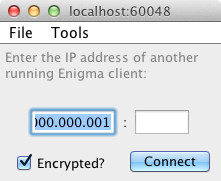
\includegraphics[scale=0.6]{./Figures/AppD/D-3.png}
\end{center}

The title bar of the window provides an important piece of information: the external port on which your server is running -- other users will need this to contact you. The port is initially random in the range $60000-60100$, however a default, fixed port can be set in Tools $>$ Options $>$ General. You do not need to do anything further to start receiving conversation requests -- other users may try and open a conversation with you once they know your IP address and port number.

The same requirements are needed for you to converse with another user -- their IP address and port number are needed, which are entered in to the input boxes in the main window. You will, however, need your key pairs to be generated first. See \textsection\ref{subsec:man_gen_keys}.

Upon connecting to a remote user or receiving a connection, a conversation window will automatically be opened.

\begin{center}
  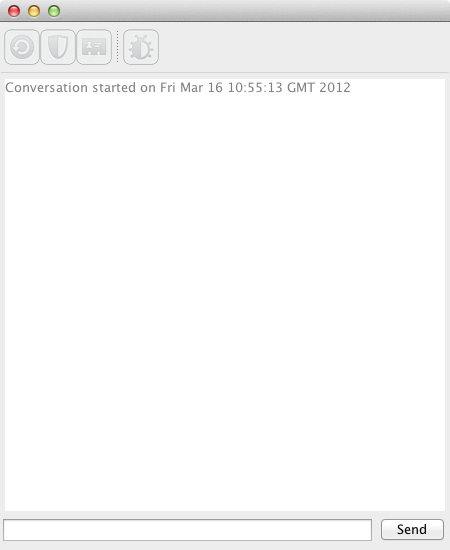
\includegraphics[scale=0.6]{./Figures/AppD/D-3b.png}
\end{center}

\section{Preferences}

The preferences window can be access through the Tools menu: Tools $>$ Options. The preferences save on change, and as such you do not need to manually click a ``save" or ``apply" button.

  \subsection{General}
  
    \paragraph{A locale} can be set, assuming the appropriate language file has been made available locally. Enigma makes use of \verb!.properties! preference files to store key/value representations of language strings that can occur within the application. See \verb!Enigma.properties! for the keys required and their associated English strings.
    
    \paragraph{The default port} can be set and so all future servers started will be run on this port.
  
  \subsection{Personal}
  
    \paragraph{A personal name} can be set which will appear to users conversing with you.
  
  \subsection{Security}
  
  \subsubsection{General}
  
    \paragraph{Unauthenticated} (and thus unencrypted) conversations are possible, however by default this option is off. Check the ``Allow Unauthenticated Conversations?" checkbox to enable this. If a user tries to connect to you without authentication when this option is on, the conversation will not be accepted.
    
    \paragraph{Certificate validation} can be turned off for testing purposes, however it is not recommended. With this setting off, man-in-the-middle attacks are possible.
  
  \subsubsection{Key Agreement}
  
    \paragraph{The default agreement method} defines the algorithm used to share keys securely between you and the remote user. This can be changed with no effect on the security of the application.
    
    \paragraph{The certificate location} must be specified after generation (if not done so automatically by the application) so that they can be shared with remote users.
    
    \paragraph{The private key location} must be specified (if not done so automatically by the application), otherwise authenticated conversations will not be possible.
    
    \paragraph{Certificate Authority} keys (both public and private) are required as the Enigma application does not make use of actual Certificate Authorities. This setting requires the location of the public key with the extension \verb!.pub! and assumes that the private key is at the same location minus that extension.
  
  \subsubsection{Cipher}
  
    \paragraph{The symmetric cipher} to be used for encryption can be set, which will also have no effect on the security of conversations.

\section{Cryptosystems}

  \subsection{Generating Keys}
  \label{subsec:man_gen_keys}
  
  Generating keys is simple and most of the work is done for you. First ensure that the location of the bundled Certificate Authority keys (public) is set in the preferences. Select ``Generate Keys..." from the Tools menu (Tools $>$ Generate Keys...) and a keypair and a certificate are automatically generated and their locations set in the preferences. No further configuration is required.
  
  Symmetric cipher keys are generated randomly for each session and cannot be manually selected through the user interface.

  \subsubsection{Notes on Maintaining Secrecy}
  
  Your private key is the very basis of the security behind sharing a cipher key and thus maintaining secrecy. If your private key is believed to be lost or stolen then a new keypair should be generated immediately.
  
  \subsection{Encrypting Conversations}
  
  Conversations are set to be encrypted by default, and the application will handle this assuming you have setup your key pairs. Unencrypted conversations may be started by either user by unchecking the ``Encrypted?" option, however both users must have the ``Allow unauthenticated conversations?" option checked if an unencrypted conversation is desired.
  
  \begin{figure}
    \centering
    
\includegraphics[scale=0.6]{./Figures/AppD/D-5-2.png}
    \caption{The toggle encryption button}
    \label{fig:toggle_enc}
  \end{figure}
  
  Throughout a conversation, assuming the ``Allow unauthenticated conversations?" preferences is checked, either user may toggle encryption on and off using the toggle button in the conversation window (see Figure \ref{fig:toggle_enc}).
  
  \begin{figure}
    \centering
    
\includegraphics[scale=0.6]{./Figures/AppD/D-5-2b.png}
    \caption{The session key regeneration button}
    \label{fig:regen_keys}
  \end{figure}
  
  If you are currently in an encrypted conversation, you are using randomly generate session keys that are automatically shared between you and the remote user. For any reason, you are able to have the session keys regenerated and sent to the remote user. See Figure \ref{fig:regen_keys}.
  
\section{Troubleshooting}

\subsection{Connection}

Upon connection, the user may receive a message "Could not connect" along with a brief description of the error.

\begin{center}
  \begin{tabular}{|l|p{5.0cm}|}
    \hline
    \textbf{Message} & \textbf{Solution} \\ \hline \hline
    Port out of range & The given port number is invalid (must be less than 65535). \\ \hline
    Connection refused & The IP address and port do not lead to a valid Enigma server. \\ \hline
    Operation timed out & The server is not accepting packets on this port. \\ \hline
    Can't find bundle for base name Enigma, locale <locale ID> & The application could not find the \verb!properties! file for your locale. Ensure that it is the same directory as the \verb!jar! file. \\
    \hline
  \end{tabular}
\end{center}

\subsection{Messages}

The protocol specifies no way to acknowledge if a message has been received, and as such if the user believes that messages are not sending they should check the local logs for the application or the console (see \textsection\ref{subsec:man_further_details}).

\subsection{Key Generation}

\begin{center}
  \begin{tabular}{|l|p{5.0cm}|}
    \hline
    \textbf{Message} & \textbf{Solution} \\ \hline \hline
    Could not find CA keys. & The Certificate Authority public/private key pair could not be found. Ensure that the location is set in Tools $>$ Options $>$ Security $>$ Key Agreement. \\ \hline
    Could not generate keys. & The keys are saved to the directory \verb!.! (the current working directory). Ensure that this directory is writeable, and that the CA keys are available. \\
    \hline
  \end{tabular}
\end{center}

For further information if this does not help, see \textsection\ref{subsec:man_further_details} as a stack trace will have been generated for any of the errors that may occur here.

If all else fails, the \verb!com.cyanoryx.uni.crypto.rsa.GenerateKeys! class can be compiled and executed to produce a key pair.

\subsection{Further Details}
\label{subsec:man_further_details}

If you launched the application through a command line shell, you will be able to view any stack traces that are printed when an error occurs. For example, in the case of a file not being found and a useful error message not being generated in-application the stack trace is a good place to start on finding out what went wrong.